\chapter{The Mindset Behind an Unforgettable Novel}

この講義は blackboard lecture ではなく interview である。したがって、その rigor は usual な意味で symbolic ではない。procedural であり、comparative であり、architectural である。最初の half-minute は、真の beginning というより overture である。そこでは、readerly presence、outlining、poetic surprise、そして description の feedback loop について、講義がやがて行き着く claims が compressed な形で聞こえてくる。ついで conversation は reset され、host が実際に始める場所、すなわち Amor Towles の descriptive precision と vocabulary への admiration から始まる。この講義には validated された board images が残っていないため、以下の displayed relations と diagrams は、visible equations の transcription ではなく、cautious な transcript-based reconstructions である。David Perell と Amor Towles の conversation は、LazyingArt LLC が curated した \emph{How You Speak and Write} コレクションに属している。

\section{Prelude、vocabularies、そして social worlds}

講義の最初の real movement は、plot、pacing、symbolism からではなく、vocabulary から始まる。Perell は Towles の socially precise な language、なかでも \emph{A Gentleman in Moscow} における French-inflected な diction に気づく。Towles はすぐに category を widen する。writer は、彼によれば、あらゆる kinds の vocabularies に interested になる。baseball、city streets、finance、ethnic neighborhoods、technical disciplines、さらには physics の language にまで。point は lexical display ではない。異なる situations は異なる verbal pressures を demand し、writer はその違いを hear するよう、ゆっくり ear を train していくのだ、ということである。

だからこそ Count が opening example として right なのだ。Count Rostov は、late nineteenth-century Europe によって formed された aristocrat である。したがって French は彼の world に belong しているのであって、decoration ではない。Towles は point をさらに sharpen する。彼自身は French を fluently に speak しないことを admit するのだ。重要なのは exhaustive mastery ではなく、social sensibility の accurate な evocation である。strategically chosen な少数の elements で、French-inflected な speech が natural であるような man の class、education、habits は bring into focus されうる。

そこから conversation は、第二の contrast へ broaden していく。\emph{A Gentleman in Moscow} が aristocratic かつ European な registers に draw しているとすれば、\emph{The Lincoln Highway} は midcentury America の sound を持たなければならない。その soundscape を prepare するために、Towles は、同じ historical moment の around で書かれたいくつかの American books へ戻る。transcript にある bibliographic sequence は多少 unstable だが、argument 自体は clear である。おおよそ同じ period の内部で書かれた books であっても、radically different な vocabularies、concerns、tonalities を carry しながら、それでも unmistakably American でありうる。language は、talent の sign であるだけではない。world を choose する way なのである。

\subsection{Question \& Answer}

\paragraph{自分自身では partly しか possess していない language-world を、どう使うのか。}

Towles の答えは modest で practical である。perfect mastery を wait しない。listen し、absorb し、real social pressure を carry する fragments を gather する。そして、write するときには、それらの fragments を authority を prove するためではなく、sensibility を evoke するために使う。standard は encyclopedic control ではない。chosen された language が character の world に belong していることである。

\section{readerly presence と description の economy}

Perell が Towles の Hopper の \emph{Nighthawks} に関する essay へ transition するとき、講義は vocabulary から effect へと shift する。彼は、自分が以前には named していなかった mood に encounter した experience を describe する。Towles は、それに deeper な aim を identify することで応じる。もっとも重要な things の一つは、reader に、book の中の experience を living しているかのように feel させることだ、と彼は言う。description が matter するのは、その state を achieve する chief means の一つだからである。

\begin{definition}
\emph{readerly presence} とは、reader が scene の inside に located していると feel し、その内部で自分を orient でき、それゆえに、そこに unfolding している thoughts、feelings、actions に interested になれる condition を意味する。
\end{definition}

Towles の causal chain は explicit なので、私たちは safely にそれを schematic に render できる。
\begin{equation}
\text{description} \longrightarrow \text{readerly presence} \longrightarrow \text{readerly engagement}.
\end{equation}
これは literal lecture mathematics ではない。spoken claim の compact notation である。description が valuable なのは、それが reader に present である feel を help するからであり、presence こそが character や event への connection を可能にするからなのだ。

\emph{A Gentleman in Moscow} における hotel は、model case を supply する。novel が decades にわたってその environment の inside に remain するからこそ、Towles は hotel の geography が early に established されねばならないことを know している。key rooms は early に vivid でなければならない。その orientation が once in place であれば、later の movement は arbitrary ではなく natural に feel される。

そこから第二の relation が follow する。
\begin{align}
\text{too little detail} &\Rightarrow \text{weak presence}, \\
\text{too much detail} &\Rightarrow \text{drag}, \\
\text{effective description} &\text{ lies in the narrow middle region.}
\end{align}
transcript は、まさにこの point で badly garbled している。だが underlying argument は firm である。description は、scene がどこでもありうるような sparse さであってはならず、同時に、reader を cold inventory に trapped させるほど specific で cumbersome でもあってはならない。writer は、space を come alive させる few elements を見つけるまで、detail を add したり remove したりするのだ。

\begin{figure}[h]
\centering
\begin{tikzpicture}[>=stealth]
\node[draw, rectangle, minimum width=3.0cm, minimum height=0.9cm] (a) at (0,0) {Describe};
\node[draw, rectangle, minimum width=3.0cm, minimum height=0.9cm] (b) at (4.0,0) {See More};
\node[draw, rectangle, minimum width=3.6cm, minimum height=0.9cm] (c) at (8.6,0) {Describe More};
\draw[->] (a) -- (b);
\draw[->] (b) -- (c);
\draw[->] (c) to[out=35,in=145] (a);
\end{tikzpicture}
\caption{Towles の iterative loop を transcript-based に schematic reconstruction したもの。description は perception を sharpen し、sharpened perception は language へ戻ってくる。}
\end{figure}

lecture の beginning にある overture は、conversation が properly に start する前からすでにこの loop を announce している。そして later には Towles が directly にそれを state する。
\begin{equation}
\text{describe} \longrightarrow \text{see more} \longrightarrow \text{describe more}.
\end{equation}
crucial な point は、description が mere report ではないということだ。ひとたび describe し始めると、私たちは more を notice し始める。more を notice すれば、language は deepen できる。

\subsection{Question \& Answer}

\paragraph{reader を bog down させずに place を vivid にするには、どれくらいの description が enough なのか。}

reader を orient させるに enough であって、彼を imprison するほどではない程度である。writer が aim するのは exhaustive totality ではない。reader に、自分がどこにいるかを know させ、その space の中を move し、その中で events が taking place していると feel させる details である。practice においてこれは、writing、rereading、adding、subtracting を通じて、どの details が actual に work をしているのかを discover することを意味する。

\section{pacing、editing、そして action のない urgency}

description の balance から、lecture は naturally に tempo へ turn する。Perell は、自分自身が repeated exposure によって sense of pace を distort されているとき、どうやって pacing を judge するのかを ask する。Towles は、その subject に別の name を与えることによって答える。Perell が really ask しているのは、editing についてなのだ、と彼は言う。

writing と editing は closely interlinked だが、same skill ではない。editing とは、すでに written したものに return し、それを colder ear で hear することである。Towles は blunt な criterion を与える。もし rereading のときに section が自分に boring に feel されるなら、それだけですでに warning sign なのだ。reader はなおさら at risk である。

key clarification は、pace と page-turning action は same thing ではない、ということだ。
\begin{equation}
\text{urgency} \neq \text{action}.
\end{equation}
classical な page-turner は、crisis、danger、event によって driven される。それは一つの art form である。literary な urgency は、もっと broader だ。reader は、character の psychology への curiosity によって、tonal pressure によって、sentence そのものの compulsion によって、あるいは outward action が minimal であっても、mind が next に何を do するのかを understand したい desire によって、forward へ draw されうる。

この distinction は、多くの pacing 論が destroy してしまう freedom を preserve する。literary novel は slow passages を contain してよい。重要なのは、その slowness が alive であるかどうかだ。もし prose がなお inward motion を generate し続けるなら、reader は still being carried しているのである。

\subsection{Question \& Answer}

\paragraph{little な external action しか起きていないとき、novel はどうやって urgency を create できるのか。}

continuation を necessary にすることによってである。reader は psychology、phrasing、tonal pressure、あるいは unresolved な question によって forward へ compelled されうる。だからこそ Towles は、target は simply speed ではないと insist する。momentum なのだ。

\section{premise、scaffolding、そして poetic mind を free にすること}

pacing の discussion のあと、Towles は一歩引いて、自分の process の architecture を describe する。これは lecture のもっとも formal な passages の一つである。彼の novels は、とても simple な premise、しばしば single sentence から begin する、と彼は言う。\emph{A Gentleman in Moscow} の場合、その premise は、おおよそ、long period of time のあいだ hotel に住む man のようなものである。もし premise に force があるなら、それは rapidly に expand する。setting、social identity、political constraint、historical span がほとんど at once に現れる。

この pipeline は、
\begin{equation}
\text{premise} \longrightarrow \text{rapid expansion} \longrightarrow \text{scaffolding} \longrightarrow \text{notebooks} \longrightarrow \text{draft} \longrightarrow \text{revision}.
\end{equation}
と要約できる。

Towles は timing について unusually specific である。
\begin{enumerate}
\item 約 \(1.5\) hours で、彼は \emph{A Gentleman in Moscow} の key elements を書き留めた。
\item およそ \(3\) days で、most of the key events の scaffolding を書いた。
\item 数年をかけて、scene investigations と visualized moments で notebooks を満たした。
\item それからはじめて、about \(1.5\) years をかけて book itself を書いた。
\item そのあとで、beginning から end までの \(2\) ないし \(3\) revision passes が来た。
\end{enumerate}

\begin{figure}[h]
\centering
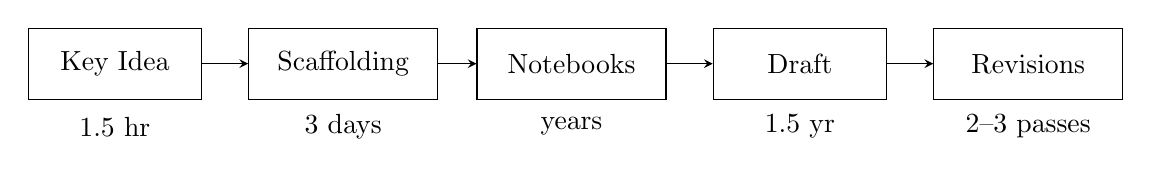
\begin{tikzpicture}[>=stealth]
\node[draw, rectangle, minimum width=2.2cm, minimum height=0.9cm] (a) at (0,0) {Key Idea};
\node[draw, rectangle, minimum width=2.4cm, minimum height=0.9cm] (b) at (2.9,0) {Scaffolding};
\node[draw, rectangle, minimum width=2.4cm, minimum height=0.9cm] (c) at (5.8,0) {Notebooks};
\node[draw, rectangle, minimum width=2.2cm, minimum height=0.9cm] (d) at (8.7,0) {Draft};
\node[draw, rectangle, minimum width=2.4cm, minimum height=0.9cm] (e) at (11.6,0) {Revisions};
\draw[->] (a) -- (b);
\draw[->] (b) -- (c);
\draw[->] (c) -- (d);
\draw[->] (d) -- (e);
\node at (0,-0.8) {$1.5$ hr};
\node at (2.9,-0.8) {$3$ days};
\node at (5.8,-0.8) {years};
\node at (8.7,-0.8) {$1.5$ yr};
\node at (11.6,-0.8) {$2$--$3$ passes};
\end{tikzpicture}
\caption{Towles の process の transcript-based schematic reconstruction。striking なのは sequence そのものだけでなく、chapter one が drafted される前にどれほど多くの structural work が already done されているかである。}
\end{figure}

notebooks が matter するのは、それが drafting stage から live uncertainty を remove するからである。Towles は、blank page の前に sitting して、real time で、room がどこにあり、誰が present しており、emotional context は何で、どんな event が起こるべきかを solve しようとしているわけではない。その much はすでに precomputed されている。drafting の question は、もっと better な question になる。この already imagined scene を life へ bring するための best language は何か、という question である。

ここから、lecture のもっとも memorable な process relation が follow する。
\begin{equation}
\text{more precomputed structure} \Rightarrow \text{less analytic load} \Rightarrow \text{more poetic freedom}.
\end{equation}
Towles は、この point を familiar な left-brain/right-brain metaphor で express する。この language は、neuroscientific というより heuristic なものとして take すべきである。argument 自体は clear だ。もし problem-solving side の mind が drafting 中ずっと fully engaged のままでなければならないなら、より dreamlike で poetic な side は damped down される。planning は、therefore、surprise の enemy ではない。それは surprise が possible になる conditions の一つなのである。

\subsection{Question \& Answer}

\paragraph{end で欲しいのが spontaneity と discovery なのに、なぜ এত इतने? Let's remove glitch. Continue smoothly.} Planning するのはなぜか。

Towles の spontaneity は、uncertainty の spontaneity ではないからである。それは、structural burdens が lifted されたあとで possible になる spontaneity なのだ。planning は surprise を replace しない。sentence の中へ surprise が enter できる space を create する。

\section{point of view、symbolism、そして character-conscious な detail}

次の local obstacle は symbolism である。ただし transcript にある host の prompt は badly corrupted している。Towles の answer は clear だ。彼は、detachable な ornaments としての symbols から begin しない。narration から begin するのである。

\emph{A Gentleman in Moscow} は third person で written されている。だが Dickens、Tolstoy、Henry James の fully omniscient mode ではない。この distinction は、図式的には
\begin{equation}
K_{\text{close third}} \subset K_{\text{omniscient third}}.
\end{equation}
と express できる。omniscient narrator は whole field を know している。すべての pasts、futures、inner lives を。Towles の narration は Count に much closer に stay する。それは、彼が notice するだろう things を tell し、彼が plausibly に feel するだろう tones をもち、彼の consciousness に belong する comic で social な inflections を帯びている。

だからこそ、resonant な detail は、first instance において symbolic insertion の matter ではない。もっと narrower で better な question を ask することの consequence であることが多い。\emph{How shall we describe the coffee?} ではなく、\emph{What would the Count notice about the coffee?} と。Towles の answer は telling である。Count は service、promptness、temperature、cuisine、things done well の dignity に notice する。これらは arbitrary な observations ではない。aristocratic habit、temperament、value、humor から arise しているのである。

講義でもっとも強い claims のひとつが、ここから follow する。後になって readers が moving や beautiful と呼ぶ passages の many は、Towles 自身が own life の中で naturally に say するような sentences ではなかった。それらは、別の consciousness を十分深く inhabit することで discover された sentences であり、その language がその person から来たかのように seem したのである。joking な line である ``Well done, Count'' は、その experience の structure を reveal している。voice が alive であるとき、sentence は character の world の inside から arrive するのだ。

lecture が full example を通して description に return する前に、それは brief だが revealing な digression を行う。Towles は chaotic artist の glamorous myth を reject し、その代わりに writing を regular work として describe する。most accomplished な writers は、彼によれば、punch the clock する。inspiration は desk において来るのであって、その before ではない。この practical claim がここで matter するのは、discussion されている all the techniques の background condition を示しているからだ。vivid sentence は discipline からの magical exemption ではないのである。

\subsection{Question \& Answer}

\paragraph{symbolism が above から mechanically に inserted されるのでないとしたら、それはどこから come するのか。}

point of view からである。ひとたび narration が genuinely にひとつの consciousness に attached されると、prose の中で visible になる things は、すでに temperament、memory、class、value、feeling によって charged されている。symbolic force はしばしばそこから emerge する。outside から separately に applied される layer としてではなく、inhabited perception の byproduct としてである。

\section{kitchen の child と、reader のための revision}

Perell はいま、deliberately exaggerated な image を経由して description に return する。ordinary perception は私たちを ``100'' までしか連れていかないかもしれないが、David Foster Wallace のような writer は ``500'' まで押し上げるのだ、と彼は rhetorically に suggest する。Towles は number scheme を own なものとして adopt はしない。だが underlying intuition は accept する。good description は seeing を change するのだ。これが、lecture のもっとも analytic な example を prepare する。

scene は simple である。young girl が early 1960s に downstairs へ来て、kitchen に入り、mother が dinner を making しているのを見る。Towles はまず、obvious な mistake を reject する。weak な writer は、period の reference material を given されると、sentence に stock markers を load したくなるかもしれない。Birdseye peas、Frigidaire、radio の Beatles。そうしたすべては historically accurate でありうる。しかもそれでも dead でありうる。problem は falsehood ではない。それが child の actually notice する things ではないことだ。それは ``1964'' を signal したくて anxious になっている outside observer が choose しそうな things なのである。

したがって Towles は、period labeling を focal perception に置き換える。seven- or eight-year-old は actual に何を見るだろうか。彼の answer において vivid なのは、brand name ではなく、package から slide して out してくる strange な frozen peas の brick であり、それが pot の上で break し、counter の across に scatter し、perhaps child が frozen pea を taste してその peculiar な texture を discover することなのだ。historical specificity は、cliche を通してではなく、consciousness を通して recover される。

\paragraph{Worked example.}

overt scene は fixed に hold する。
\begin{equation}
S = \text{child enters the kitchen at dinner time}.
\end{equation}
いま hidden state を vary する。
\begin{align}
H_1 &= \text{the mother has just discovered her husband's infidelity}, \\
H_2 &= \text{the mother has just committed her own infidelity}.
\end{align}
visible room は almost unchanged のままかもしれない。だが realized prose はそうではありえない。
\begin{align}
S + H_1 &\Rightarrow D_1, \\
S + H_2 &\Rightarrow D_2, \\
D_1 &\neq D_2.
\end{align}
ここで \(D_1\) と \(D_2\) は、furniture が moved したから differ するのではない。diction、tempo、gesture、atmosphere が changed したから differ するのである。

\begin{figure}[h]
\centering
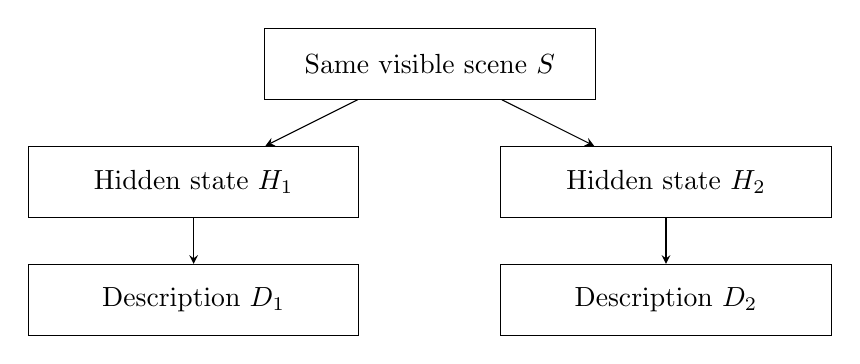
\begin{tikzpicture}[>=stealth]
\node[draw, rectangle, minimum width=4.2cm, minimum height=0.9cm] (s) at (0,2.0) {Same visible scene $S$};
\node[draw, rectangle, minimum width=4.2cm, minimum height=0.9cm] (h1) at (-3.0,0.5) {Hidden state $H_1$};
\node[draw, rectangle, minimum width=4.2cm, minimum height=0.9cm] (h2) at (3.0,0.5) {Hidden state $H_2$};
\node[draw, rectangle, minimum width=4.2cm, minimum height=0.9cm] (d1) at (-3.0,-1.0) {Description $D_1$};
\node[draw, rectangle, minimum width=4.2cm, minimum height=0.9cm] (d2) at (3.0,-1.0) {Description $D_2$};
\draw[->] (s) -- (h1);
\draw[->] (s) -- (h2);
\draw[->] (h1) -- (d1);
\draw[->] (h2) -- (d2);
\end{tikzpicture}
\caption{kitchen scene の transcript-based schematic reconstruction。overt scene は fixed のままでも、mother の hidden history が tone、pace、language を change させうる。}
\end{figure}

Towles の point は、さらに subtler である。child は、何が happened したのかを consciously には know していないかもしれない。それでも mother の behavior は、その hidden state の trace を carry していなければならない。so that later、truth が discovered されたとき、reader は return して、it was all there と say できるのである。focal consciousness には解釈できなくとも sense はできる knowledge で、scene はすでに vibrating していたのだ。

iterative logic が、ここで greater force とともに戻ってくる。私たちは first に accurately observe する。それから words を choose する。ついで、visible なものだけでなく、household の emotional field、class setting、regional context、historical moment をも include する larger truth へ向かって revise する。scene は merely kitchen ではない。this family の、この pressures の下にある、この kitchen なのだ。

\subsection{Question \& Answer}

\paragraph{cliche を avoid しながら、それでも scene を historically specific かつ emotionally loaded にするにはどうすればよいか。}

decade に label を貼る historian のように write することを refuse することである。代わりに、この age の、この situation のこの perceiver が actual に何を notice するだろうかを ask する。そして hidden state が、beneath から scene の language と tempo を reshape することを allow する。historical specificity は、expected markers の pile を通してではなく、lived perception を通して enter するのである。

Towles はこの example を、そのまま drafting の ethics に turn する。first draft は、自分一人のために written される、と彼は言う。fascinations、digressions、vanities、odd pleasures が proliferate するのを、彼は restraint なしに allow する。後になって初めて、lens を reverse し、reader 側から covenant を read する。
\begin{equation}
\text{first draft for self} \longrightarrow \text{revision for reader}.
\end{equation}
この second phase は marketing exercise ではない。obligation である。もし reader が money を、そしてもっと importantly には time を与えているなら、writer はその return として economy を owe している。redundancy、boredom、cliche、purely private な indulgence は cut されねばならない。したがって revision は largely subtractive である。それは prose を leaner、sharper、そして story の actual needs に truer なものにする。この stage で Towles はまた、editors や trusted literary friends を含む thoughtful readers の small circle に turn し、その responses によって book を outside から test するのである。

\subsection{Question \& Answer}

\paragraph{ourselves のためではなく reader のために revise するとき、exactly 何が change するのか。}

judgment の axis が change する。first draft では、private fascination が expand することを allow する。revision では、何が story に belong し、何が merely writer の whim を flatter しているだけなのかを問う。result は、abundance から economy へ、self-directed な exploration から reader-centered な form への movement である。

\section{craft、reading、poetry、manifestos、doors、そして New York}

revision から、lecture は teachability へ broaden する。Towles は formal teacher として speak することに resist する。だが彼の answer は nonetheless precise である。もし teaching が repeated practice、disciplined exposure、craft の elements に対する growing command を意味するのだとすれば、多くの things は taught しうる。彼は explicitly に long list を name する。
\begin{itemize}
\item plot,
\item setting,
\item dialogue,
\item tone of voice,
\item perspective,
\item metaphor,
\item simile,
\item allusion,
\item allegory.
\end{itemize}
decisive な word は genius ではなく repetition である。人は again and again writing することによって command を gain する。そして Towles はさらに重要な demand を加える。young writers は many perspectives から write すべきだ。different genders、classes、ages、regions、countries、sensibilities は、craft を fixed ではなく variable なものとして rediscover することを writer に force する。``how to describe a room'' のための single formula などない。room は、それに enter する mind とともに change するからである。

同じ principle は reading を govern する。Towles は、自分にとって reading と writing は childhood から onward ほとんど simultaneous だったと describe する。彼は、first-grade の teacher が poet を classroom に bring し、signed books を receiving した experience を remember している。この memory が matter するのは、origin の moment において、language、performance、authorship を join しているからである。later には、reading は more analytic になる。彼は pen を手に read する。structure を study する。structure について write する。books を comparative に、historically に扱う reading group に join する。point は passive admiration ではない。investigation なのである。

ひとつの revealing な heuristic がここに現れる。history は、Towles によれば、すべての greatness を preserve することには poor だが、mediocre なものを discard することには comparatively good である。shorthand form にすれば、
\begin{equation}
\text{corpus at } t \longrightarrow \text{filtered canon at } t+50.
\end{equation}
となる。これは rule of thumb であって law ではない。だが彼や彼の friends が、older authors をしばしば読む理由を説明してくれる。past が every greatness を capture したからではなく、time が some filtering を already done してくれているからである。

Towles は sentence level にも linger する。Roth の paragraph は、ときに one consciousness から another へ、あるいは briefly omniscience へ、almost invisibly に move しながら rupture を起こさない。その kind の fluid viewpoint movement は、dangerous であるがゆえに powerful である。mishandled なら reader を jar させる。well に handled されれば、narrative possibility を enlarge する。

poetry に関する remarks は、balance の problem へ戻ってくる。too much poetic indeterminacy が relief なしに sustained されれば、reader は exhausted してしまう。novel は therefore、orientation を stabilize するときと、language が dream、ambiguity、resonance へ move することを allow するときを know していなければならない。同じ balance が、別の register で、manifestos に関する彼の remarks にも return する。彼に interest があるのは doctrine as such ではなく、verbal energy である。manifestos は declarative で、staccato で、self-assured で、action-oriented である。それらは、too much explanation によって自分を slow down しない。
\begin{equation}
\text{high declaration density} + \text{low explanatory drag} \Rightarrow \text{manifesto energy}.
\end{equation}

lecture の final metaphor は、こうした late themes を single test へ gather する。promising な idea とは、doors を open するものだ。writer は one small thing を見るか、あるいは one compressed premise を持つ。そして immediately に many rooms が appear し始める。
\begin{equation}
\text{premise} \Rightarrow \text{many possible continuations}.
\end{equation}
この metaphor によって、conversation は New York で close できるようになる。Towles にとって New York は、ethnicity や nationality の melting pot であるだけではない。passions の melting pot である。journalism、cuisine、dance、finance、law、advertising、theatre、その他の pursuits は、ambitious な young people を same city の中へ draw する。result は、overlapping aspiration の density である。その density が city に strange electricity を与え、そして Towles の imagination において New York が setting としてだけでなく、narrative possibility の engine として function する理由を explain するのである。

\subsection{Question \& Answer}

\paragraph{passing observation のまま remain するのではなく、novel へ grow するに enough rich な idea とは、何によって判定されるのか。}

Towles の test は branching power である。good premise は、almost immediately に rooms を open し始める。もし一つの idea が、quickly に many scenes、many pressures、many characters、many routes forward を suggest するなら、writer はその richness を、それを fully に write down する前から feel するのである。

\section{まとめ}

この lecture には literal な board mathematics はない。だが、きわめて useful な意味で rigorous である。それは、ひとつの chain of necessities を与えてくれる。vocabulary は world に belong しなければならない。description は presence を create しなければならない。presence は engagement を support しなければならない。editing は urgency と mere speed を distinguish しなければならない。planning は analytic burden を reduce しなければならず、そうすることで surprise が sentence の inside で occur できるようになる。point of view は meaningful detail を consciousness の inside から generate しなければならない。revision は private abundance を readerly economy へ convert しなければならない。そして最後に reading は、structure、tone、sentence movement、historical judgment が continually に writer 自身の practice に return してくる、reciprocal な apprenticeship にならなければならない。

lecture の order を in mind に keep しておけば、whole discussion は hang together する。それは language で open し、presence へ narrow し、pacing へ turn し、process へ widen し、point of view へ drill down し、kitchen example を through して scene へ reenter し、それから revision、teachability、reading、poetry、manifestos、door-opening premises、そして New York の urban ecology へと outward に open し直す。result は、inspiration の doctrine ではない。imaginative freedom がいかに build されるかについての disciplined な account なのである。